\section{多変量解析}
多変量解析とは多変量データを統計的に扱う手法である。
扱うデータの科学的知識に基づいた特徴量抽出に加え、実データの統計的な性質を考慮した
特徴量抽出も様々な分野で行われている。
この章では脳波解析で用いられている多変量解析について紹介し、
その有用性と限界について考察する。

\subsection{Principal Component Analysis(PCA)}
Principal Component Analysis(PCA)は特徴量抽出手法として幅広い分野で活用されている。
簡単のため時間平均が\(0\)の多次元信号\(x(t)\in \mathbb R^D\)に対してPCAによる特徴抽出を考える。
PCAでは変換行列\(W^T \in \mathbb R^{D \times D}\)を左から作用させ、特徴量
\begin{equation}
    z(t)=W^Tx(t) \in \mathbb R^D
\end{equation}
を獲得するが、この際、\(z(t)\)の各成分が互いに無相関になるように\(W\)を決定する。
\(z(t)\)が無相関となるためには、その分散共分散行列\(\Sigma_z=\mathbb E[z(t)z^T(t)]\)が対角行列になることが要請される。
ここで\(x(t)\)の分散共分散行列を\(\Sigma_x=\mathbb E[x(t)x^T(t)]\)とすると、\(z(t)\)の分散共分散行列\(\Sigma_z\)について
\begin{eqnarray}
    \Sigma_z & = & \mathbb E[z(t)z^T(t)] \nonumber \\
    & = & \mathbb E[W^Tx(t)x^T(t)W] \nonumber \\
    & = & W^T \mathbb E[x(t)x^T(t)]W \nonumber \\
    & = & W^T \Sigma_x W
    \label{var}
\end{eqnarray}
と表すことができる。(\ref{var})が対角行列になるような\(W\)は、\(\Sigma_x\)の固有値分解によって求まる。
実数信号の分散共分散行列は一般に正定値実対称行列となっており、直交行列によって固有値分解が可能である。
また、固有値は必ず正の値となる。これらの数学的な扱いやすさからPCAは非常に広く普及している。
\begin{figure}[htbp]
    \begin{minipage}{0.5\hsize}
     \begin{center}
      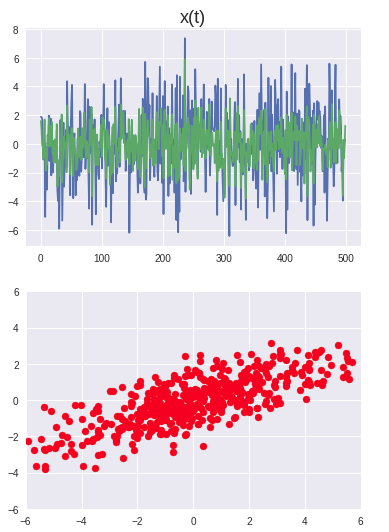
\includegraphics[width=70mm]{images/x(t).png}
     \end{center}
     \caption{x(t)の波形と散布図}
     \label{fig:x(t)}
    \end{minipage}
    \begin{minipage}{0.5\hsize}
     \begin{center}
      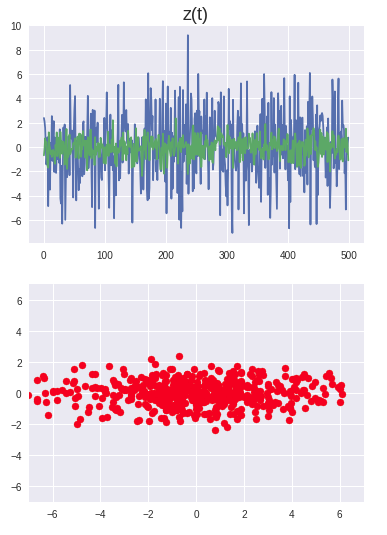
\includegraphics[width=70mm]{images/z(t).png}
     \end{center}
     \caption{z(t)の波形と散布図}
     \label{fig:z(t)}
    \end{minipage}
\end{figure}

\begin{figure}
    \centering
    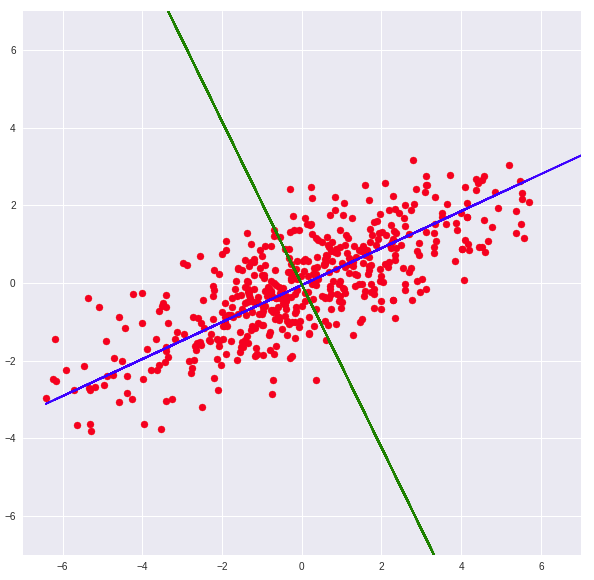
\includegraphics[width=12cm]{images/z=Wx.png}
    \caption{PCAによって得られる基底}
    \label{fig:z=Wx}
\end{figure}
図\ref{fig:x(t)}は人工的に作成した2次元波形\(x(t)\)と各成分の散布図である。
この\(x(t)\)に対してPCAを用いると、
図\ref{fig:z(t)}に示す\(z(t)\)が得られ、散布図から
\(z(t)\)の各成分は無相関となっていることが確認できる。
図\ref{fig:z=Wx}は\(x(t)\)に対してPCAを施した場合に得られる新たな直交基底を表しており、
\(z(t)\)は新たな直交基底に\(x(t)\)を射影したものに他ならない。
PCAでは基底を取り直すことで各成分が無相関な信号を獲得でき、
その結果、新たに得られた信号の各成分がどのような意味を持つのかを考察しやすくなる。

しかし、応用上は単に基底を取り直すことを目的とするケースは少ない。
通常は固有値分解によって求まった固有ベクトル(新たな基底)を全て利用するのではなく、
値の大きな固有値に属する固有ベクトル\(w\)を\(d(<D)\)個選び、
\(W_{d} = (w_1, \cdots, w_d)\)によって変換行列を構成することで、
\begin{equation}
    z(t)=W_{d}^Tx(t) \in \mathbb R^d
    \label{reduction}
\end{equation}
と次元削減を行う。
値の大きな固有値に属する固有ベクトルによって基底を構成することは、
\(W_d\)による基底の元で、信号の分散(あるいは振幅)が最大化されることを要請することと等価である。
また、射影先での分散最大化に伴い、(\ref{reduction})での変換行列\(W_d\)は、
元々の信号\(x(t)\)と、\(x(t)\)を\(\mathbb R^D\)の部分空間
\(\mathbb R^d\)へ射影した信号\(z(t)\)との二乗誤差を最小化する変換行列となっている。


以上からPCAは、元々の信号\(x(t)\)の情報損失を二乗誤差の意味で最小限に抑えながら、
射影先で大きな変動を有し、かつ各成分が無相関となる特徴量\(z(t)\)を抽出する。しかし、脳波への応用を考える上ではPCAの性質は必ずしも有効には働かない。
運動想起BCIを考える上では、脳波に含まれる全ての情報の中から識別したい身体部位に関する情報のみを抽出する必要がある。
この場合、脳波信号のごく一部のみが重要である可能性があり、射影先で大きな分散を持つような信号となっているかは定かではないためである。




\subsection{Indipendent Component Analysis(ICA)}
Indipendent Component Analysis(ICA)はPCAを発展させた比較的新しい信号解析手法である。
ICAはPCAと同様に変換行列\(W^T \in \mathbb R^{D \times D}\)を左から作用させ、特徴量
\begin{equation}
    z(t)=W^Tx(t) \in \mathbb R^D
\end{equation}
を獲得するが、この際、\(z(t)\)の各成分が互いに独立になるように\(W\)を決定する。
独立性は無相関性の十分条件であり、PCAに比べて\(z(t)\)により強い条件を要請する。
PCAでは無相関性が固有値分解という数学的によく知られた問題と関連していたが、独立性は簡単な問題への定式化は困難であるため、
通常は独立性を測る目的関数を設定し、勾配法などの逐次最適化法を用いる。
最も普及している求解アルゴリズムはFastICAとして知られており、
独立性の必要条件である無相関性を要請した後、独立性を最大化することで解を得る。
図\ref{fig:ica_pca}にPCAとICAの振る舞いをトイデータを用いて比較を掲載する。
図\ref{fig:ica_pca}のbase vectors of ICA and PCAから分かるようにICAで得られる基底は直交するとは限らない。
また、PCAの基底の大きさは等しく\(1\)であり正規直交基底を構築するが、ICAでは正規性も持つとは限らない。
\begin{figure}
    \centering
    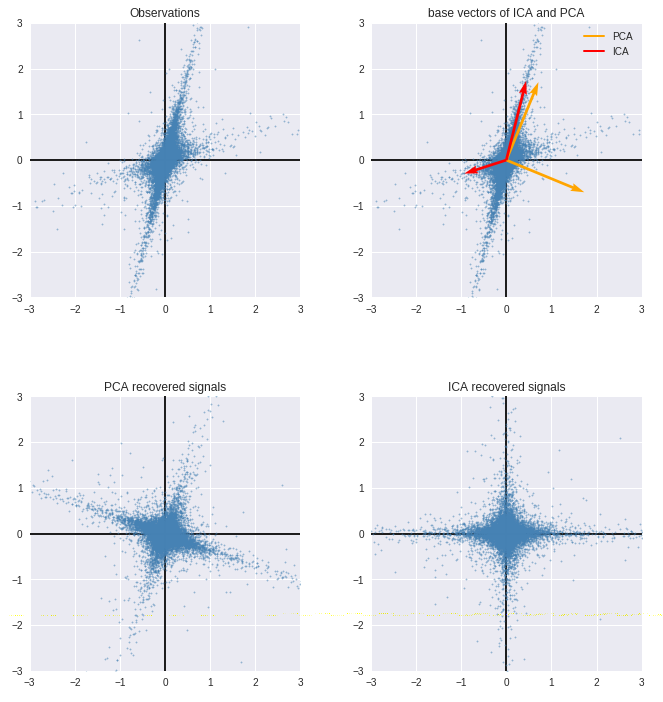
\includegraphics[width=15cm]{images/ica_pca.png}
    \caption{無相関な基底を得るPCAと独立な基底を獲るICAの比較}
    \label{fig:ica_pca}
\end{figure}


脳波への応用では、脳波計測時に混入した脳波以外の信号(筋電位、眼電位など)が脳波とは統計的に独立であると考え、
脳波以外の信号成分を除去する目的で利用される。一方で運動想起BCIにおいて身体部位に関する脳波成分を直接抽出することはPCA同様に難しい。
筋電などの場合、脳波と独立であるという仮定は妥当であり、
かつ振幅が目視可能なほど脳波に比べて大きくなる。従って、ICAによって分解された独立な成分から筋電などを見分けるのは比較的容易である。
しかし、一方で身体部位に関する脳波成分がその他のあらゆる脳波と独立であるかは定かではなく、仮に独立であった場合にも分解された信号から
目視によって特定することは困難であると推察される。

\subsection{Blind Source Separation(BSS)}
上記ではPCAとICAが次元削減として用いられることを見た。
一方でこれらの手法はBlind Source Separation(BSS)問題の解法として解釈されることも多いため、
ここで簡単に述べておく。
まず信号源\(s(t)\ \in \mathbb R^d\)を直接観測できない場合に、
\(D\)個のセンサで\(x(t) \in \mathbb R^D\)という信号を観測したとする。
このとき、観測信号\(x(t)\)のみから信号源\(s(t)\)を推定する問題がBSS問題である。
計測機器や環境に応じて、信号源\(s(t)\)は何らかの変換\(f(\cdot)\)を受けて観測されると考えられる。
従って\(x(t)\)は
\begin{equation}
    x(t)=f(s(t))
\end{equation}
と表記できる。このときに観測に伴う変換\(f(\cdot)\)が線形変換\(A\)であると仮定した場合、
\begin{equation}
    x(t)=As(t)
    \label{eq:bss1}
\end{equation}
と表記することができ、BSS問題は\(x(t)\)から\(A\)と\(s(t)\)を同時に推定する問題であると見なせる。
ここで仮に適当な線形変換によって、観測信号\(x(t)\)を
\begin{equation}
    z(t)=Wx(t)
    \label{eq:bss2}
\end{equation}
と変換することを考える。
\(W\)を上手く選ぶことに成功すれば、\(z(t)=Wx(t) \simeq s(t)\)となることが期待できる。
ここで\(D=d\)、すなわち信号源の次元と観測信号の次元が一致している場合を考える。
このとき(\ref{eq:bss1})において、
\(A\)が正則であるとし、
\begin{equation}
    s(t)=A^{-1}x(t)
\end{equation}
と表すことが可能になる。従って、(\ref{eq:bss2})の\(W\)を\(W=A^{-1}\)とすることができれば、
\begin{equation}
    z(t)=Wx(t)=A^{-1}x(t)=s(t)
\end{equation}
と信号源を求めることが可能である。
ただし、\(z(t)=s(t)\)となる\(W\)が存在するとしても、
既知の\(x(t)\)に対して未知の\(W,s(t)\)を求めようとしている状況に変わりはなく、BSS問題は基本的に不良設定問題である。
また、実データでは信号源と観測信号の次元が一致しない場合が多く\(A\)は逆行列を持たないため、
状況はより複雑である場合が多い。通常はBSS問題を解くためには何らかの条件を追加するか、
正則化の手法を導入する必要がある。
PCAやICAは信号源\(s(t)\)が各成分について無相関あるいは独立であると仮定することで条件式を追加し、
観測信号\(x(t)\)から条件式を満たすような\(W\)と\(z(t)\)を求め、
\(z(t)\)が信号源\(s(t)\)の良い近似になっていると考えるBSS問題の解法の一種である。

PCAとICAのBSS問題への振る舞いを確認するために、トイデータによる実験結果を図\ref{fig:bss}に示す。
周波数の異なる2つの正弦波と1つのノコギリ波にそれぞれガウスノイズを加算した信号源(図\ref{fig:bss}のTrue Sources)
を準備し、適当な線形変換を施して観測信号(図\ref{fig:bss}のObservations)とする。
図\ref{fig:bss}のICA recoverd signalsがFastICAによって推定された信号源に適当なゲインを加えたものであり、
図\ref{fig:bss}のPCA recoverd signalsがPCAによって推定された信号源に適当なゲインを加えたものである。
ICAでは周波数の異なる正弦波とノコギリ波を明確に分解できており、
信号源に近い波形が得られていることが確認できるが、
PCAでは信号源と異なる信号が得られている。
PCAの振る舞いは各成分を無相関にしつつ、射影先で分散を最大化するような基底を求めるため
ノコギリ波と位相が一致している正弦波を1つの成分に集約してしまっている。

\begin{figure}
    \centering
    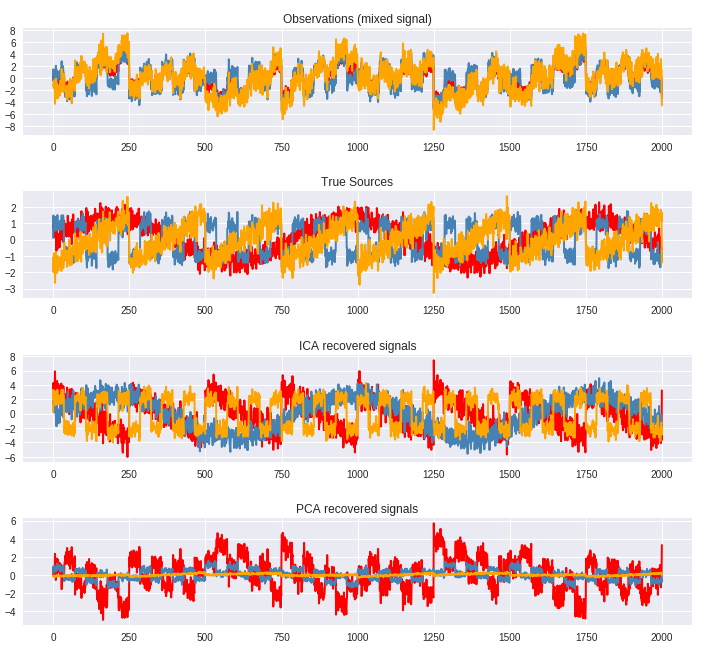
\includegraphics[width=15cm]{images/bss.png}
    \caption{BSS問題に対するPCAとICA}
    \label{fig:bss}
\end{figure}

トイデータによる実験ではICAがBSS問題に対して有効に働くことが確認できるが、
本来信号源がどのようなものであるかは未知であるため、
信号源推定が正しく行われたかを確認するのは実データでは困難である。
運動想起BCIを想定して脳波にBSS問題を適用する場合には、観測された信号\(x(t)\)
から脳波信号の根源である\(s(t)\)を復元することを目的とするが、ICAによって推定された信号源の
いずれの成分が運動想起と関連しているのかを判別するのは極めて難しい。
ただし、脳波と筋電では波形が明らかに異なるため、筋電と脳波が独立であるという仮定を用いて
ICAによって筋電成分を取り出すことは可能である。
一般に、不良設定問題であるBSS問題に対しては何らかの仮定を置かざるを得なく、
複雑な脳波に対して適切な仮定を設けることが重要な課題となる。